\documentclass[Royal,times,sageh]{sagej}

\usepackage{moreverb,url,natbib, multirow, tabularx}
\usepackage[colorlinks,bookmarksopen,bookmarksnumbered,citecolor=red,urlcolor=red]{hyperref}



% tightlist command for lists without linebreak
\providecommand{\tightlist}{%
  \setlength{\itemsep}{0pt}\setlength{\parskip}{0pt}}

% From pandoc table feature
\usepackage{longtable,booktabs,array}
\usepackage{calc} % for calculating minipage widths
% Correct order of tables after \paragraph or \subparagraph
\usepackage{etoolbox}
\makeatletter
\patchcmd\longtable{\par}{\if@noskipsec\mbox{}\fi\par}{}{}
\makeatother
% Allow footnotes in longtable head/foot
\IfFileExists{footnotehyper.sty}{\usepackage{footnotehyper}}{\usepackage{footnote}}
\makesavenoteenv{longtable}




\begin{document}


\setcitestyle{aysep={,}}

\title{Análisis de los determinantes en la fecundidad de las mujeres en
Bolivia}

\runninghead{}

\author{Valentina Valdez Vega\affilnum{1}}

\affiliation{\affilnum{1}{Estudiante de la carrera de ``Economía e
Inteligencia de Negocios'', Universidad Católica Boliviana ``San
Pablo''}}



\begin{abstract}
hola
\end{abstract}

\keywords{Fecundidad, Bolivia, Regresión Logit, Regresión Poisson;}

\maketitle

\section{Introducción}\label{introducciuxf3n}

Según los resultados de la última Encuesta de Demografía y Salud (EDSA
2023), realizada por el Instituto Nacional de Estadística (INE), se
observó una disminución en la tasa de fecundidad en Bolivia. La tasa de
fecundidad en 2023 llegó a 2,1 en comparación a la tasa de 2,9 que se
obtuvo en la pasada encuesta EDSA de 2016. Esta caída en la fecundidad
no es una sorpresa para países dentro de la región latinoamericana y
puede ser relacionada con cambios culturales, nuevas expectativas de
vida por parte de la población joven y la creciente inserción al mercado
laboral de la población femenina. Por otra parte, se ha visto una fuerte
asociación respecto a elevados niveles de pobreza, especialmente en
hogares monoparentales o rurales (UNPD, 2015), y lo que se entiende como
una alta fecundidad\footnote{Según la definición por el UNPD (2015), se
  define alta fecundidad como haber tenido cuatro o más hijos nacidos
  vivos.}.

La Encuesta de Demografía y Salud (EDSA) constituye una fuente de
información relevante al momento de obtener indicadores de salud y
demografía a nivel nacional, que posteriormente ayudarán el diseño de
políticas públicas implementadas en el país boliviano. La EDSA ofrece
información importante para analizar la fecundidad en Bolivia, ya que
permite vincular los patrones reproductivos con variables
sociodemográficas, culturales y de salud, además de gozar de una
cobertura a nivel nacional. De esta forma, esta encuesta actúa como
fuente de información esencial para la construcción de modelos
predictivos que identifican los factores más significativos asociados a
la fecundidad de mujeres adultas en edad fértil \footnote{Según la
  definición de la EDSA (2023) considera una mujer adulta en edad fértil
  a aquellas mujeres entre 20 y 49 años.} (INE \& UNFPA, 2023).

En este sentido, resulta necesario analizar los factores determinantes
en la fecundidad de las mujeres en Bolivia, para así poder entender de
mejor forma por qué existe una tendencia a la baja respecto a la tasa de
fecundidad y el número de hijos por mujer. Para tal efecto, es posible
utilizar modelos estadísticos de regresión tales como la regresión
logística y la regresión Poisson. Por un lado, la regresión logística
permite estimar la probabilidad de ocurrencia de una variable binaria a
partir de variables independientes, lo cual resulta clave para
identificar factores de fecundidad. Por otro lado, la regresión Poisson
permite examinar cómo varía la fecundidad en cuanto al número de hijos
según características individuales como la edad, nivel educativo,
actividad económica o pertenencia étnica (Schultz, 2006).

\section{Objetivos}\label{objetivos}

\subsection{Objetivo General}\label{objetivo-general}

Analizar los factores determinantes en la fecundidad de las mujeres
adultas y el número de hijos nacidos vivos por mujer adulta en edad
fértil en Bolivia, a través de modelos de regresión logit y Poisson.

\subsection{Objetivos Específicos}\label{objetivos-especuxedficos}

\begin{itemize}
\item
  Desarrollar el modelo de regresión logístico para explicar los
  determinantes de la fecundidad en las mujeres adultas en Bolivia a
  partir de los datos obtenidos en la encuesta EDSA 2023.
\item
  Desarrollar el modelo de regresión logístico para explicar los
  determinantes de la alta fecundidad en las mujeres adultas en Bolivia
  a partir de los datos obtenidos en la encuesta EDSA 2023.
\item
  Desarrollar el modelo de regresión de Poisson para modelar el número
  total de hijos nacidos vivos de las mujeres adultas en edad fértil a
  partir de los datos obtenidos en la encuesta EDSA 2023.
\item
  Evaluar el efecto de los determinantes socioeconómicos y demográficos
  tales como el nivel de pobreza, educación y lugar de residencia en la
  fecundidad de las mujeres adultas y el número de hijos nacidos vivos
  de las mujeres en edad fértil en Bolivia, basado en el enfoque de
  Schultz (Schultz, 2006).
\item
  Emplear pruebas de bondad de ajuste convencionales, como ser la
  devianza y el criterio de información de Akaike (AIC), para la
  evaluación de los modelos desarrollados en la presente investigación.
\end{itemize}

\section{Motivación}\label{motivaciuxf3n}

La fecundidad constituye uno de los indicadores demográficos más
relevantes dentro de la dinámica de un país, ya que influye de forma
directa en el crecimiento de una población, la estructura por edades y,
como consecuencia, permite diseñar políticas sociales y económicas como
sean requeridas. Como menciona Schultz (2006), el estudio de la
fecundidad no solo se reserva a una decisión propia de una familia o
persona, si no que tiene fuertes implicaciones económicas y sociales
dentro de una sociedad. A partir de esto, se refuerza la influencia de
la fecundidad como un factor esencial del desarrollo de un país y la
importancia de comprender los factores que determinan la fecundidad
dentro de una economía, para poder entender su comportamiento.

En Bolivia, tomando en cuenta los resultados presentados en la Encuesta
de Demografía y Salud, se ha observado que persisten diferencias
geográficas, étnicas y socioeconómicas que inciden en los patrones de
fecundidad de las mujeres. Como se observa en la figura 1 y se mencionó
en la sección 1, los resultados posteriores a la recolección de
información para la EDSA (en sus dos versiones 2016 y 2023) muestran una
tendencia a la baja en lo que compete a la tasa global de
fecundidad\footnote{La tasa global de fecundidad se entiende como el
  número promedio de hijos que tendrá una mujer a lo largo de su vida
  fértil, comprendida entre los 15 a 49 años.} a nivel Bolivia. En ambos
casos, se observa una disminución de 3,5 a 2,9 para el año 2016, y una
reducción a 2,1 para el año 2023. Sin embargo, comparando con otros
países de América Latina, se observa que desde el 2008 la tasa global de
fecundidad boliviana se mantiene mayor respecto a países como Ecuador,
Brasil y Chile. Aunque, como región, en todos los países se observa una
tendencia decreciente. Esta reducción en la tasa global de fecundidad
conduce a una población con una proporción menor de jóvenes, lo cual
genera desafíos para la fuerza laboral, la sostenibilidad de los
sistemas sociales y afecta directamente el crecimiento poblacional.

\begin{figure}

{\centering 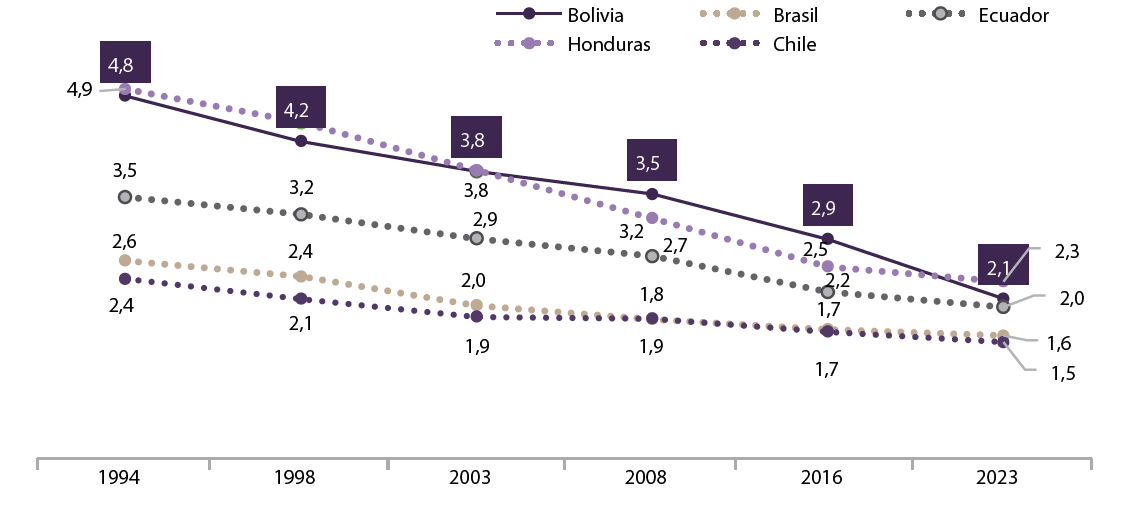
\includegraphics[width=1\linewidth]{imagenes/foto1} 

}

\caption{Evolución de la Tasa Global de Fecundidad en Bolivia y países de la región.\\\textit{Fuente: INE, 2023 - en base a la ENDSA 1994, 1998, 2003 y 2008, EDSA 2016 y 2023, y Banco Mundial 2022.}}\label{fig:unnamed-chunk-1}
\end{figure}

De esta forma, la investigación surge como un aporte dentro de la
necesidad de generar evidencia empírica que contribuya a entender los
determinantes sociales, económicos y culturales de la fecundidad en
Bolivia, utilizando la Encuesta de Demografía y Salud (EDSA 2023), que
además se enfoque en analizar componentes actuales dentro de esta
temática. Para que así, se pueda entender de mejor forma la disminución
en la tasa global de fecundidad observada en los últimos años, y se
puedan plantear políticas o programas que respondan a estos resultados.
Igualmente, la investigación emplea los modelos de regresión logit y
Poisson, los cuales en base a su connotación teórica y práctica permiten
llevar a cabo el estudio.

\section{Marco Teórico}\label{marco-teuxf3rico}

\subsection{Fecundidad y Fertilidad}\label{fecundidad-y-fertilidad}

La fecundidad y la fertilidad son conceptos centrales en la demografía
debido a ser indicadores relevantes al analizar la dinámica demográfica
y el crecimiento de una población. Aunque frecuentemente son usados como
sinónimos, tienen significados distintos. Mientras que la fertilidad
alude a la capacidad biológica de tener hijos, la fecundidad se refiere
al número efectivo de nacimientos (Rodríguez Vignoli, 2014). De esta
forma, la fecundidad se convierte en una variable clave en la
planificación de políticas públicas debido a su impacto en la estructura
poblacional y en la demanda de servicios educativos, sanitarios,
laborales y sistemas de seguridad social (CEPAL, 2020).

Un aporte relevante al estudio de la fertilidad es realizado por T.P.
Schultz (2006), quien establece una relación inversa entre el ingreso y
la fecundidad. Según su análisis, a medida que aumenta el ingreso y la
educación de las mujeres, la fecundidad tiende a disminuir, lo que
responde tanto a la mayor participación femenina en el mercado laboral
como a un cambio en las preferencias familiares respecto a la
planificación reproductiva. Este enfoque ha sido retomado en estudios
posteriores para explicar patrones reproductivos en países en
desarrollo. En el caso de América Latina, ha atravesado una transición
demográfica significativa donde se observó una reducción en las tasas de
fecundidad en la región. Sin embargo, esta disminución no ha sido
homogénea, ya que persisten niveles elevados en ciertos grupos
poblacionales, especialmente en zonas rurales y entre mujeres con menor
acceso a educación y/o servicios (Schultz, 2006).

Por otro lado, como Schultz (2006) menciona en su capítulo ``Fertility
and Income'', las variables determinantes de la fecundidad femenina
pueden ser fundamentadas bajo un enfoque económico y provenir de la
evidencia y la teoría microeconómica. Ante esto, las principales
variables que afectan la fecundidad según Schultz son: el ingreso, la
educación, el uso de anticonceptivos y la planificación familiar, la
mortalidad infantil, el entorno social y cultural y otras variables
exógenas que pueden tomar en cuenta la edad de la mujer y el estado
conyugal.

\subsection{Determinantes de la fecundidad según
Schultz}\label{determinantes-de-la-fecundidad-seguxfan-schultz}

El ingreso es entendido de dos formas: la primera se refiere al ingreso
derivado del capital físico, como ser la tierra, que tiende a aumentar
la fecundidad, pues incrementa el consumo familiar y el valor financiero
inmediato de tener más hijos, y la segunda toma en cuenta el ingreso
derivado del capital humano de la mujer, es decir los ingresos propios
de la mujer, el cual tiende a reducir la fecundidad, debido al mayor
costo de oportunidad del tiempo de la mujer con el hecho de llegar a ser
madre. Por otro lado, la educación de la madre es un factor relevante ya
que mayores años de escolaridad femenino están asociados de forma
negativa con la tasa de fecundidad. La educación incrementa el costo de
oportunidad de la maternidad y repercute de manera positiva en el status
y la autonomía de la mujer (Enríquez-Canto, Ortiz-Romaní \&
Ortiz-Montalvo, 2017).

En lo que respecta a los métodos anticonceptivos y la planificación
familiar, Schultz denota que el acceso a métodos anticonceptivos reduce
de forma efectiva la fecundidad para una pareja. Así mismo, Schultz
indica que dicho aspecto está íntimamente ligado a la educación y la
salud reproductiva dentro de una pareja. Por otro lado, al hablar de la
mortalidad infantil, una reducción en este indicador genera que la
esperanza por tener más hijos disminuya para una familia, lo cual reduce
la fecundidad. De esta forma, se enfatiza la influencia de la
supervivencia infantil en las decisiones reproductivas (Schultz, 2006).

Las normas sociales y culturales sobre familia y fecundidad, así como el
entorno social, condicionan las expectativas sobre el tamaño ideal del
hogar; aunque Schultz se centra más en factores económicos, su análisis
reconoce esta dimensión. Adicionalmente, es necesario mencionar la
relevancia de esta última variable en el estudio de la fecundidad, ya
que se asocia la reducción de las tasas de fecundidad a nivel de país e
incluso a nivel mundial con el cambio dentro de las expectativas
personales y/o profesionales dentro de los jóvenes y los nuevos ideales
del tamaño familiar. Mismas variables están intrínsicamente relacionadas
con la sociedad y cultura moderna (Enríquez-Canto, Ortiz-Romaní \&
Ortiz-Montalvo, 2017).

Finalmente, pese a que Schultz no menciona a la edad y el estado
conyugal de una mujer como determinantes causal principales en su
modelo, estas variables pueden ser cruciales en términos del horizonte
fértil y el momento de decisión de reproducción para una familia. Como
tal, Schultz analiza la fecundidad acumulada por edades específicas,
añadiendo así de forma implícita a la edad como parte de la estructura
de oportunidades de fecundidad. Respecto al estado conyugal, el hecho de
estar en pareja formal (ya se en matrimonio o convivencia) facilita o
incrementa la probabilidad de tener hijos. A su vez, la decisión de
formar pareja también puede verse influida por variables económicas,
como el ingreso esperado o la educación.

\subsection{Alta fecundidad}\label{alta-fecundidad}

La alta fecundidad se refiere a niveles por encima del reemplazo
poblacional, que aproximadamente resulta ser 2.1 hijos por mujer.
Entendiendo al reemplazo poblacional como el número promedio de hijos
que una mujer necesita tener para que, en promedio, cada generación
reemplace a la anterior en una población sin crecimiento ni disminución.
Ciertos autores como Bongaarts (2015) y UNFPA (2023) toman en cuenta a
la alta fecundidad para valores de la tasa global de fecundidad mayores
a cuatro. En contextos como Bolivia, este fenómeno está asociado con
bajos niveles educativos, pobreza, desigualdad de género, y acceso
limitado a servicios tanto de salud sexual como reproductiva (UNFPA,
2023). De esta manera, como mencionan estudios recientes, se destaca que
la alta fecundidad puede constituir una barrera para el desarrollo
económico y la equidad, particularmente cuando se presenta en mujeres
adolescentes o en grupos marginados (Binstock, 2021).

\subsection{Regresión logística}\label{regresiuxf3n-loguxedstica}

La regresión logística es una técnica estadística utilizada para modelar
relaciones entre una variable dependiente dicotómica (binaria 1/0) y un
conjunto de variables independientes que pueden ser cualitativas o
cuantitativas. A diferencia de la regresión lineal, este modelo estima
la probabilidad de ocurrencia de un evento binario, como presencia y
ausencia o éxito y fracaso, mediante la función logística, la cual
garantiza que los valores predichos se encuentren entre 0 y 1.

Desde 2010, la regresión logística ha mantenido un rol central clave en
investigaciones aplicadas dentro de la epidemiología, ciencias sociales
y economía, como herramienta para obtener resultados importantes según
los objetivos que se tengan. Según Hosmer, Lemeshow y Sturdivant (2013),
la interpretación de los coeficientes de una regresión logística permite
entender el cambio de las chances (odds) en la probabilidad de un evento
por unidad de cambio en la variable predictora, lo cual resulta
especialmente útil en contextos donde se busca analizar las
posibilidades de ocurrencia de un suceso. En lo que compete al análisis
de los determinantes de la fecundidad, los modelos estadísticos como la
regresión logística son adecuados a la hora de modelar variables
dicotómicas como ``tener hijos o no''.

\subsection{Regresión Poisson}\label{regresiuxf3n-poisson}

La Regresión Poisson es un modelo no lineal que toma en cuenta a una
variable cualitativa discreta como la variable dependiente, en general
modela y predice variables de conteo. Esta regresión parte de la
distribución Poisson que precisamente se utiliza para analizar conteos o
números de eventos en un intervalo dado. De esta forma, en estos casos,
la variable dependiente toma más de dos valores discretos no negativos
(números del 0, 1, 2, en adelante). La distribución Poisson es utilizado
comúnmente para modelar el número de ocurrencias de cierto evento en un
medio continuo (generalmente hace referencia al tiempo), por ejemplo, es
útil para modelar conteos como el número de hijos que tiene una mujer
adulta en edad fértil. Siendo de esta forma un instrumento correcto para
el presente estudio.

\section{Descripción del dataset}\label{descripciuxf3n-del-dataset}

Los datos que se usaron para trabajar con el modelado, tanto de la
regresión logística como de la regresión Poisson, fueron obtenidos a
través de la última versión de la Encuesta de Demografía y Salud (EDSA),
realizada por el INE en 2023. La encuesta EDSA forma parte de las
investigaciones que se realizan de forma periódica y a nivel nacional,
con el fin de proporcionar información para el cálculo referente a los
principales indicadores de salud y demografía como ser la fecundidad,
salud materna e infantil, mortalidad infantil y de niñez, vacunación,
estado nutricional de los menores de seis años y anticoncepción.
Posteriormente, esta información se convierte en el pilar fundamental
para formular y evaluar el diseño de políticas públicas y programas que
se implementen en Bolivia bajo el Plan de Desarrollo Económico y Social
(PDES).

La EDSA 2023 fue realizada bajo cuatro cuestionarios temáticos:
cuestionario hogar, cuestionario mujer, cuestionar hombre y el
cuestionario de primera infancia, donde cada uno de ellos aborda
preguntas diferentes enfocados en la población a la que se encuesta.
Para motivos del análisis de datos de la investigación, se utilizaron
los datos provenientes del cuestionario mujer, donde se obtiene
información respectiva a los datos personales y preferencias de
reproducción de las mujeres, y también la información del cuestionario
hogar para obtener el ingreso de la familia (esta variable será
aproximada mediante el quintil de riqueza).

Así, las variables\footnote{El diccionario de variables de la EDSA 2023
  puede ser encontrado en el catálogo ANDA.} seleccionadas de forma
inicial para realizar la regresión logit y Poisson son detalladas en la
tabla 1. El motivo por el cual se seleccionaron estás variables va en
línea con la teoría descrita por Schultz (2006) sobre los factores
económicos y sociales que influyen en la tasa de fecundidad. En el caso
de determinante de mortalidad infantil, no existe una variable que
recoja esta información proveniente de la EDSA 2023, por lo que no será
tomada en cuenta.

\subsubsection{Tabla 1. Variables utilizadas en el
estudio}\label{tabla-1.-variables-utilizadas-en-el-estudio}

\begin{longtable}[]{@{}
  >{\raggedright\arraybackslash}p{(\columnwidth - 4\tabcolsep) * \real{0.2422}}
  >{\raggedright\arraybackslash}p{(\columnwidth - 4\tabcolsep) * \real{0.1366}}
  >{\raggedright\arraybackslash}p{(\columnwidth - 4\tabcolsep) * \real{0.6211}}@{}}
\toprule\noalign{}
\begin{minipage}[b]{\linewidth}\raggedright
Factor (según Schultz)
\end{minipage} & \begin{minipage}[b]{\linewidth}\raggedright
Código variable
\end{minipage} & \begin{minipage}[b]{\linewidth}\raggedright
Descripción
\end{minipage} \\
\midrule\noalign{}
\endhead
\bottomrule\noalign{}
\endlastfoot
\textbf{Variable dependiente} & ms02\_0208 & Número de hijos nacidos
vivos \\
\textbf{Ingreso} & qriqueza & Quintil de riqueza del hogar \\
& ms08\_0809 & Si trabajó de forma remunerada durante la semana
pasada \\
\textbf{Educación} & niv\_ed & Nivel de educación alcanzado general \\
& aestudio & Años de estudio alcanzados por la encuestada \\
\textbf{Métodos anticonceptivos y planificación familiar} & ms02\_0276 &
Si recibió información sobre educación sexual \\
& cono\_algmet & Conocimiento de métodos anticonceptivos \\
& actmaconcep\n\_cme\_m & Si actualmente usa algún método
anticonceptivo \\
\textbf{Entorno social y cultural} & pertenece & Pertenencia a una
nación o pueblo indígena (hecho en base a la variable ms01\_0108) \\
& idioma\_orig & Si el primer idioma aprendido en la niñez es un idioma
originario (hecho en base a la variable ms01\_0106) \\
& departamento & Departamento de residencia \\
& region & Región geográfica de residencia (altiplano, valle o llano) \\
& area & Área de residencia (urbana o rural) \\
\textbf{Edad} & ms01\_0101a & Edad cumplida en años \\
\textbf{Estado conyugal} & actuni\_m & Si actualmente se encuentra en
unión con una pareja \\
\end{longtable}

\emph{Fuente: Elaboración propia en base a ENDSA, 2023.}

Respecto a las variables idioma\_orig y pertenece se hizo una
transformación de las variables ms01\_0106 (idioma o lengua que se
aprendió a hablar en la niñez) y ms01\_0108 (nación o pueblo originario
al que pertenece). Así, la variable idioma\_orig toma en cuenta si la
mujer aprendió a hablar un idioma originario en su niñez como el éxito,
para de esta forma conocer si la mujer nació en una familia originaria.
En el caso de la variable pertenece se toma en cuenta si la mujer
pertenece a un pueblo o nación originaria como el éxito, para conocer si
se considera parte de un pueblo indígena.

\subsection{Regresión logit}\label{regresiuxf3n-logit}

La regresión logit para los determinantes de la fecundidad se toma en
cuenta a las mujeres mayores a 19 años. La variable dependiente en este
caso corresponde a una transformación sobre la variable ms02\_0208,
donde se toma en cuenta una variable dicotómica (denominada hijos) con
el éxito cuando el número de hijos es por lo menos uno y el fracaso
cuando el número de hijos es igual a cero.

En el caso de la regresión logit para analizar la alta fecundidad
también se realizó transformación sobre la variable ms02\_0208, pero en
este caso el éxito se tomó cuando el número de hijos es por lo menos
cuatro y el fracaso cuando el número de hijos es menor a cuatro.

\subsection{Regresión Poisson}\label{regresiuxf3n-poisson-1}

La regresión Poisson se toma en cuenta a las mujeres mayores a 19 años,
donde la variable dependiente en este caso corresponde a la variable
ms02\_0208, que representa el número de hijos vivos de una mujer.

\section{Metodología}\label{metodologuxeda}

\section{Resultados y análisis}\label{resultados-y-anuxe1lisis}

\section{Conclusiones y
recomendaciones}\label{conclusiones-y-recomendaciones}

\bibliographystyle{sageh}
\bibliography{biblio}


\end{document}
